
\section{Technical details}
\label{sec:proofs}
\subsection{Proof of \Cref{prop:bellman-expectation}}
\label{sec:proof-bell-expect}
\begin{proof}
	Thanks to the introduction of the augmented spaces $\ocS, \ocA$ and dynamics $\augmentedtransition$, this proof is the same as that in classical \glspl{MOMDP}.
	\begin{align*}
	\oV^{\budgetedpolicy}(\os) &\eqdef \expectedvalue\left[ \augmentedreturn^{\budgetedpolicy} \condbar \ov{s_0} = \os\right] \\
	&=\sum_{\oa\in\ocA} \probability{\oa_0 = \oa \condbar\ov{s_0} = \os} \expectedvalue\left[ \augmentedreturn^{\budgetedpolicy} \condbar \ov{s_0} = \os, \oa_0 = \oa\right]\\
	&= \sum_{\oa\in\ocA} \budgetedpolicy(\oa | \os) \oQ^{\budgetedpolicy}(\os,\oa).
	\end{align*}
	
	\begin{align*}
	\oQ^{\budgetedpolicy}(\os, \oa) &\eqdef \expectedvalue\left[\sum_{t=0}^\infty \discountfactor^t \augmentedreward(\os_t, \oa_t)\condbar \ov{s_0} = \os, \ov{a_0} = \oa\right] \\
	&= \augmentedreward(\os, \oa) + \sum_{\os'\in\ocS}\probability{\os_1 = \os' \condbar\ov{s_0} = \os, \ov{a_0} = \oa}\cdot \expectedvalue\left[\sum_{t=1}^\infty \discountfactor^t \augmentedreward(\os_t, \oa_t)\condbar \ov{s_1} = \os'\right] \\
	&= \augmentedreward(\os, \oa) + \discountfactor\sum_{\os'\in\ocS}\augmentedtransition\left(\os' \condbar\os, \oa\right) \expectedvalue\left[\sum_{t=0}^\infty \discountfactor^t \augmentedreward(\os_t, \oa_t) \condbar \ov{s_0} = \os'\right] \\
	&= \augmentedreward(\os, \oa) + \discountfactor\sum_{\os'\in\ocS}\augmentedtransition\left(\os' \condbar\os, \oa\right) \oV^{\budgetedpolicy}(\os').
	\end{align*}
	
	\paragraph{Contraction of $\abo^{\budgetedpolicy}$.}
	Let $\budgetedpolicy\in\policies, \oQ_1, \oQ_2\in(\Real^2)^{\ocS\ocA}$.
	\begin{align*}
	\forall \os\in\ocS, \oa\in\ocA,\quad \left|\abo^{\budgetedpolicy} \oQ_1(\os,\oa) - \abo^{\budgetedpolicy} \oQ_2(\os,\oa)\right| &= \left|\discountfactor\expectedvalueover{\substack{\os'\sim\augmentedtransition(\os'|\os,\oa) \\ \oa'\sim\budgetedpolicy(\oa'|\os')}} \oQ_1(\os',\oa') - \oQ_2(\os',\oa')\right|\\
	&\leq \discountfactor\left\|\oQ_1-\oQ_2\right\|_\infty.
	\end{align*}
	Hence, $\left\|\abo^{\budgetedpolicy} \oQ_1 - \abo^{\budgetedpolicy} \oQ_2 \right\|_\infty \leq \discountfactor\left\|\oQ_1-\oQ_2\right\|_\infty$
	
	According to the Banach fixed point theorem \citep{Banach1922}, $\abo^{\budgetedpolicy}$ admits a unique fixed point.
	It can be easily verified that $\oQ^{\budgetedpolicy}$ is indeed this fixed point by combining the two Bellman Expectation equations~\eqref{eq:bellman_expectation}.
	
\end{proof}

\subsection{Proof of \Cref{thm:bellman-optimality}}
\label{sec:proof-bell-optim}

\begin{proof}
    Let $\os, \oa \in \ocA\times\ocS$. For this proof, we consider potentially non-stationary policies $\budgetedpolicy=(\rho, \budgetedpolicy')$, with $\rho\in\cM(\ocA)$, $\budgetedpolicy'\in\cM(\ocA)^\Natural$. The results will apply to the particular case of stationary optimal policies, when they exist.
    \begin{align}
        \Qr[^\star](\os, \oa) &=  \max_{\rho, \budgetedpolicy'} \Qr[^{\rho, \budgetedpolicy'}](\os', \oa') \label{eq:pthm_def}\\
        &= \max_{\rho, \budgetedpolicy'} \reward(s, a) + \discountfactor \sum_{\os'\in\ocS} \augmentedtransition(\os' | \os, \oa) \Vr[^{\rho, \budgetedpolicy'}](\os') \label{eq:pthm_exp}\\
        &= \reward(s, a) + \discountfactor \sum_{\os'\in\ocS}  \augmentedtransition(\os' | \os, \oa) \max_{\rho, \budgetedpolicy'} \sum_{\oa'\in\ocA} \rho(\oa' | \os')\Qr[^{\budgetedpolicy'}](\os', \oa') \label{eq:pthm_marg}\\
        &= \reward(s, a) + \discountfactor \sum_{\os'\in\ocS}  \augmentedtransition(\os' | \os, \oa) \max_\rho\sum_{\oa'\in\ocA}\rho(\oa' | \os')\max_{\budgetedpolicy'\in\policies_a(\os')}\Qr[^{\budgetedpolicy'}](\os', \oa') \label{eq:pthm_max}\\
        &= \reward(s, a) + \discountfactor \sum_{\os'\in\ocS}  \augmentedtransition(\os' | \os, \oa) \max_\rho\expectedvalueover{\oa'\sim\rho}\Qr[^\star](\os', \oa') \label{eq:pthm_marg_def2}
    \end{align}
    where $\budgetedpolicy = (\rho, \budgetedpolicy')\in\policies_a(\os)$ and $\budgetedpolicy'\in\policies_a(\os')$.

    This follows from:
    \begin{enumerate}
        \item[\eqref{eq:pthm_def}.] Definition of $\oQ^{\star}$.
        \item[\eqref{eq:pthm_exp}.] Bellman Expectation expansion from \Cref{prop:bellman-expectation}.
        \item[\eqref{eq:pthm_marg}.] Marginalisation on $\oa'$.
        \item[\eqref{eq:pthm_max}.] \begin{itemize}
            \item Trivially $\max_{\budgetedpolicy'\in\policies_a(\os')} \sum_{\oa'\in\ocA} \cdot \leq \sum_{\oa'\in\ocA} \max_{ \budgetedpolicy'\in\policies_a(\os)} \cdot$.
            \item Let $\ov{\budgetedpolicy}\in\argmax_{\budgetedpolicy'\in\policies_a(\os')} \Qr[^{\budgetedpolicy'}](\os', \oa')$, then:
            \begin{align*}
                \sum_{\oa'\in\ocA}\rho(\oa'|\os')\max_{\budgetedpolicy'\in\policies_a(\os')}\Qr[^{\budgetedpolicy'}](\os', \oa') &= \sum_{\oa'\in\ocA}\rho(\oa'|\os')\Qr[^{\budgetedpolicy'}](\os', \oa') \\
                &\leq  \max_{\budgetedpolicy'\in\policies_a(\os')} \sum_{\oa'\in\ocA}\rho(\oa'|\os')\Qr[^{\budgetedpolicy'}](\os', \oa').
            \end{align*}
        \end{itemize}
        \item[\eqref{eq:pthm_marg_def2}.] Definition of $\oQ^{\star}$.
    \end{enumerate}

    Moreover, the condition $\budgetedpolicy=(\rho, \budgetedpolicy')\in\policies_a(\os)$ gives
    \begin{equation*}
        \expectedvalueover{\oa'\sim\rho} \Qc[^{\star}](\os, \oa) = \expectedvalueover{\oa'\sim\rho} \Qc[^{\budgetedpolicy'}](\os, \oa) = \Vc[^{\budgetedpolicy}](\os) \leq \budget.
    \end{equation*}

    Consequently, $\budgetedpolicy_\text{greedy}(\cdot; \oQ^{\star})$ belongs to the $\argmax$ of \eqref{eq:pthm_marg_def2}, and in particular:
    \begin{equation*}
        \Qr[^{\star}](\os, \oa) = r(\os, \oa) + \discountfactor \sum_{\os'\in\ocS}  P(\os' | \os, \oa) \expectedvalueover{\oa'\sim\budgetedpolicy_\text{greedy}(\os', \oQ^{\star})} \Qr[^{\star}](\os', \oa').
    \end{equation*}

    The same reasoning can be made for $\Qc[^\star]$ by replacing $\max$ operators by $\min$, and $\policies_a$ by $\policies_r$.
\end{proof}


\subsection{Proof of \Cref{prop:greedy_optimal}}
\label{sec:proof-greedy-optim}
\begin{proof}
    Notice from the definitions of $\abo^{\star}$ and $\abo^{\budgetedpolicy}$ in \eqref{eq:bellman-optimality} and \eqref{eq:bellman_expectation_operator} that $\abo^{\star}$ and $\abo^{\budgetedpolicy_\text{greedy}(\cdot;\oQ^{\star})}$ coincide on $\oQ^{\star}$. Moreover, since $\oQ^{\star} = \abo^{\star}\oQ^{\star}$ by \Cref{thm:bellman-optimality}, we have: $\abo^{\budgetedpolicy_\text{greedy}(\cdot;\oQ^{\star})} \oQ^{\star} = \abo^{\star} \oQ^{\star} = \oQ^{\star}$.
    Hence, $\oQ^{\star}$ is a fixed point of $\abo^{\budgetedpolicy_\text{greedy}(\cdot;\oQ^{\star})}$, and by \Cref{prop:bellman-expectation} it must be equal to $\oQ^{\budgetedpolicy_\text{greedy}(\cdot;\oQ^{\star})}$

    To show the same result for $\oV^{\star}$, notice that
    \begin{equation*}
        \oV^{\budgetedpolicy_\text{greedy}(\oQ^{\star})}(\os) = \expectedvalueover{\oa\sim\budgetedpolicy_\text{greedy}(\oQ^{\star})}\oQ^{\budgetedpolicy_\text{greedy}(\oQ^{\star})}(\os,\oa) = \expectedvalueover{\oa\sim\budgetedpolicy_\text{greedy}(\oQ^{\star})}\oQ^{\star}(\os,\oa).
    \end{equation*}
    By applying the definitions of $\oQ^{\star}$ and $\budgetedpolicy_\text{greedy}$, we recover the definition of $\oV^{\star}$.
\end{proof}

\subsection{Proof of \Cref{thm:contraction}}
\label{sec:proof-contraction}
\begin{proof}
	In the trivial case $|\cA| = 1$, there exits only one policy $\budgetedpolicy$ and $\abo = \abo^\budgetedpolicy$, which is a contraction by \Cref{prop:bellman-expectation}.
	
	In the general case $|\cA| \geq 2$, we can build the following counter-example.
	
	Let $(\cS, \cA, P, R_r, R_c)$ be a \gls{BMDP}.
	For any $\epsilon > 0$, we define $\oQ_\epsilon^1$ and $\oQ_\epsilon^2$ as
	\begin{align*}
	\oQ_\epsilon^1(\os,\oa) =
	\begin{cases}
	(0, 0), & \text{if } a = a_0 \\
	\left(\frac{1}{\discount}, \epsilon\right), & \text{if } a \neq a_0
	\end{cases}\\
	\oQ_\epsilon^2(\os,\oa) =
	\begin{cases}
	(0, \epsilon), & \text{if } a = a_0 \\
	\left(\frac{1}{\discount}, 2\epsilon\right), & \text{if } a \neq a_0
	\end{cases}
	\end{align*}
	Then, $\|\oQ_1-\oQ_2\|_\infty = \epsilon$.
	$\oQ_\epsilon^1$ and $\oQ_\epsilon^2$ are represented in \Cref{fig:concavity_example}.
	
	\begin{figure}[tp]
		\centering
		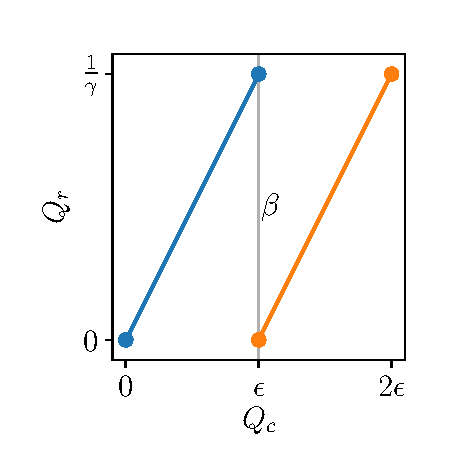
\includegraphics[width=0.4\textwidth]{img/concavity_example.pdf}
		\caption{Representation of $\oQ_\epsilon^1$ (blue) and $\oQ_\epsilon^2$ (yellow)}
		\label{fig:concavity_example}
	\end{figure}
	
	But for $\oa=(a,\budgetaction)$ with $\budgetaction = \epsilon$, we have
	\begin{align*}
	\|\abo \oQ_\epsilon^1(\os, \oa) - \abo \oQ_\epsilon^2(\os, \oa)\|_\infty &= \discount\left\|\expectedvalueover{\os'\sim\augmentedtransition(\os'|\os,\oa)} \expectedvalueover{\oa'\sim\budgetedpolicy_\text{greedy}(\oQ^1_\epsilon)}\oQ^1_\epsilon(\os',\oa') - \expectedvalueover{\oa'\sim\budgetedpolicy_\text{greedy}(\oQ^2_\epsilon)}\oQ^2_\epsilon(\os',\oa')\right\|_\infty \\
	&= \discount\left\|\expectedvalueover{\os'\sim\augmentedtransition(\os'|\os,\oa)}\left(\frac{1}{\discount}, \epsilon\right) - (0, \epsilon)\right\|_\infty \\
	&= \discount\frac{1}{\discount} = 1
	\end{align*}
	Hence, 
	\begin{align*}
	\|\abo \oQ_\epsilon^1 - \abo \oQ_\epsilon^2\|_\infty &\geq 1 = \frac{1}{\epsilon} \|\oQ_1-\oQ_2\|_\infty
	\end{align*}
	
	In particular, there does not exist $L>0$ such that
	$$\forall \oQ_1,\oQ_2\in(\Real^2)^{\ocS\ocA}, \|\abo \oQ^1 - \abo \oQ^2\|_\infty \leq L \|\oQ^1 - \oQ^2\|_\infty$$
	In other words, $\abo$ is not a contraction for $\|\cdot\|_\infty$.
\end{proof}

\subsection{Proof of \Cref{thm:contractivity-smooth}}
\label{sec:contraction-with-smooth}

\begin{remark}
	\begin{leftbar}[remarkbar]
	This proof makes use of insights detailed in the proof of \Cref{prop:bftq_pi_hull} (\Cref{sec:proof_pi_hull}), which we recommend the reader to consult first.
	\end{leftbar}
\end{remark}

\begin{proof}
	We now study the contractivity of $\abo^{\star}$ when restricted to the functions of $\cL_{\discountfactor}$ defined as follows:
    \begin{equation}
    \cL_{\discountfactor} = \left\{\begin{array}{cc}
   \oQ\in(\Real^2)^{\ocS\ocA}\text{ s.t. }\exists L<\frac{1}{\discountfactor}-1: \forall \os\in\ocS,\oa_1,\oa_2\in\ocA,   \\
   |\Qr(\os,\oa_1) - \Qr(\os,\oa_2)| \leq L|\Qc(\os,\oa_1) - \Qc(\os,\oa_2)|
    \end{array}\right\}.
    \end{equation}
    That is, for all state $\os$, the set $\oQ(\os, \ocA)$ plot in the $(\Qc,\Qr)$ plane must be the \emph{graph} of a $L$-Lipschitz function, with $L<1/\discountfactor-1$.

    We impose such structure for the following reason: the counter-example presented above prevented contraction because it was a pathological case in which the slope of $\oQ$ can be arbitrary large. As a consequence, when solving $\Qr[^\star]$ such that $\Qc[^\star]=\budget$, a vertical slice of a $\|\cdot\|_\infty$ ball around $\oQ_1$ (which must contain $\oQ_2$) can be arbitrary large as well.


    We denote $\text{Ball}(\oQ,R)$ the ball of centre $\oQ$ and radius $R$ for the $\|\cdot\|_\infty$-norm:
    \begin{equation*}
        \text{Ball}(\oQ,R) = \{\oQ'\in(R^2)^{\ocS\ocA}: \|\oQ-\oQ'\|_\infty \leq R\}.
    \end{equation*}

    We give the three main steps required to show that $\abo^{\star}$ restricted to $\cL_{\discountfactor}$ is a contraction. Given $\oQ^1, \oQ^2\in\cL_{\discountfactor}$, show that:

    \begin{enumerate}
        \item $\oQ^2\in\text{Ball}(\oQ^1,R)\implies\cF^2\in\text{Ball}(\cF^1, R), \forall\os\in\ocS$, where $\cF$ is the top frontier of the convex hull of undominated points, as defined in~\Cref{sec:proof_pi_hull}.
        \item $\oQ\in\cL_{\discountfactor} \implies \cF$ is the graph of a $L$-Lipschitz function, $\forall\os\in\ocS$.
        \item taking the slice $\Qc=\budget$ of a ball $\text{Ball}(\cF,R)$ with $\cF$ $L$-Lipschitz results in an interval on $\Qr$ of range at most $(L+1)R$
    \end{enumerate}
	
	These three steps will allow us to control $\Qr[^{2\star}] - \Qr[^{1\star}]$ as a function of $R = \|\oQ^2-\oQ^1\|_\infty$.

    \paragraph{Step 1}

    We want to show that if $\oQ^1$ and $\oQ^2$ are close, then $\cF^1$ are $\cF^2$ are close as well in the following sense:
    \begin{align}
        \cF^2\in\text{Ball}(\cF^1, R) &\iff d(\cF^1, \cF^2) \leq R \iff \max_{q^2\in\cF^2}\min_{q^1\in\cF^1}\|q^2-q^1\|_\infty \leq R.
        \label{eq:ball-set}
    \end{align}

    Assume $\oQ^2\in\text{Ball}(\oQ^1,R)$, we show by contradiction that $\cF^2 \in \text{Ball}(\cF^1, R)$. Indeed, assume there exists $q^1\in \cF^1$ such that $\cF^2 \cap \text{Ball}(q^1, R) = \emptyset$. Denote $q^2$ the unique point of $\cF^2$ such that $q^2_c = q^1_c$. By construction of $q^1$, we know that $\|q^1-q^2\|_\infty > R$. There are two possible cases:
    \begin{itemize}
        \item $q^2_r > q^1_r$: this also directly implies that $q^2_r > q^1_r + R$. But $q^2\in\cF^2$, so there exist $q^2_1, q^2_2\in Q^{2},\lambda\in\Real$ such that $q^2 = (1-\lambda)q^2_1 + \lambda q^2_2$. But since $\oQ^2\in \text{Ball}(\oQ^1, R)$, there also exist $q_1^1, q^1_2\in \oQ^1$ such that $\|q^1_1-q^2_1\|_\infty \leq R$ and $\|q^1_2-q^2_2\|_\infty \leq R$, and in particular $q^1_{1r}\geq q^2_{1r}-R$ and $q^1_{2r}\geq q^2_{2r}-R$. But then, the point $q^{1'}=(1-\mu)q^1_1 + \mu q^1_2$ with $\mu=(q^2_c-q^1_{1c})/(q^2_{2c}-q^1_{1c})$ verifies $q^{1'}_c = q^1_c$ and $q^{1'}_r \geq q^2_r - R > q^1_r$ which contradicts the definition of $q_1\in\cF^1$ as defined in \eqref{eq:top-frontier}.
        \item $q^2_r < q^1_r$: then the same reasoning can be applied by simply swapping the indexes 1 and 2.
    \end{itemize}

    % We start by showing this result for $\cC^2(Q^{1-})$ and $\cC^2(Q^{2-})$ as defined in \Cref{sec:proof_pi_hull}:
    % Let $\os\in\ocS$ and $q^2\in\cC^2(Q^{2-})$, $\exists\lambda\in[0,1], \oa_1,\oa_2\in\ocA: q^2 = (1-\lambda)Q^2(\os,\oa_1) + \lambda Q^2(\os,\oa_2)$. Define $q^1 = (1-\lambda)Q^1(\os,\oa_1) + \lambda Q^1(\os,\oa_2)$. Then
    % \begin{align*}
    %     \|q^2-q^1\|_\infty &= \|(1-\lambda)(Q^2(\os,\oa_1) - Q^1(\os,\oa_1)) + \lambda (Q^2(\os,\oa_2) - Q^1(\os,\oa_2))\|_\infty\\
    %     &\leq  (1-\lambda)\|Q^2(\os,\oa_1) - Q^1(\os,\oa_1)\|_\infty + \lambda \|Q^2(\os,\oa_2) - Q^1(\os,\oa_2)\|_\infty\\
    %     &\leq (1-\lambda)R+\lambda R = R
    % \end{align*}

    % It remains to show that when taking the top frontiers of the convex sets $\cC^2(Q^{1-})$ and $\cC^2(Q^{2-})$, they remain at a distance of at most $R$.

    We have shown that $\cF^2 \in \text{Ball}(\cF^1, R)$.
    This is illustrated in \Cref{fig:contraction_lips_hull}: given a function $\oQ^1$, we show the locus $\text{Ball}(\oQ_1,R)$ of $\oQ^2$. We then draw $\cF^1$ the top frontier of the convex hull of $\oQ^1$ and alongside the locus of all possible $\cF^2$, which belong to a ball $\text{Ball}(\cF^1, R)$.

    \begin{figure}[ht]
        \centering
        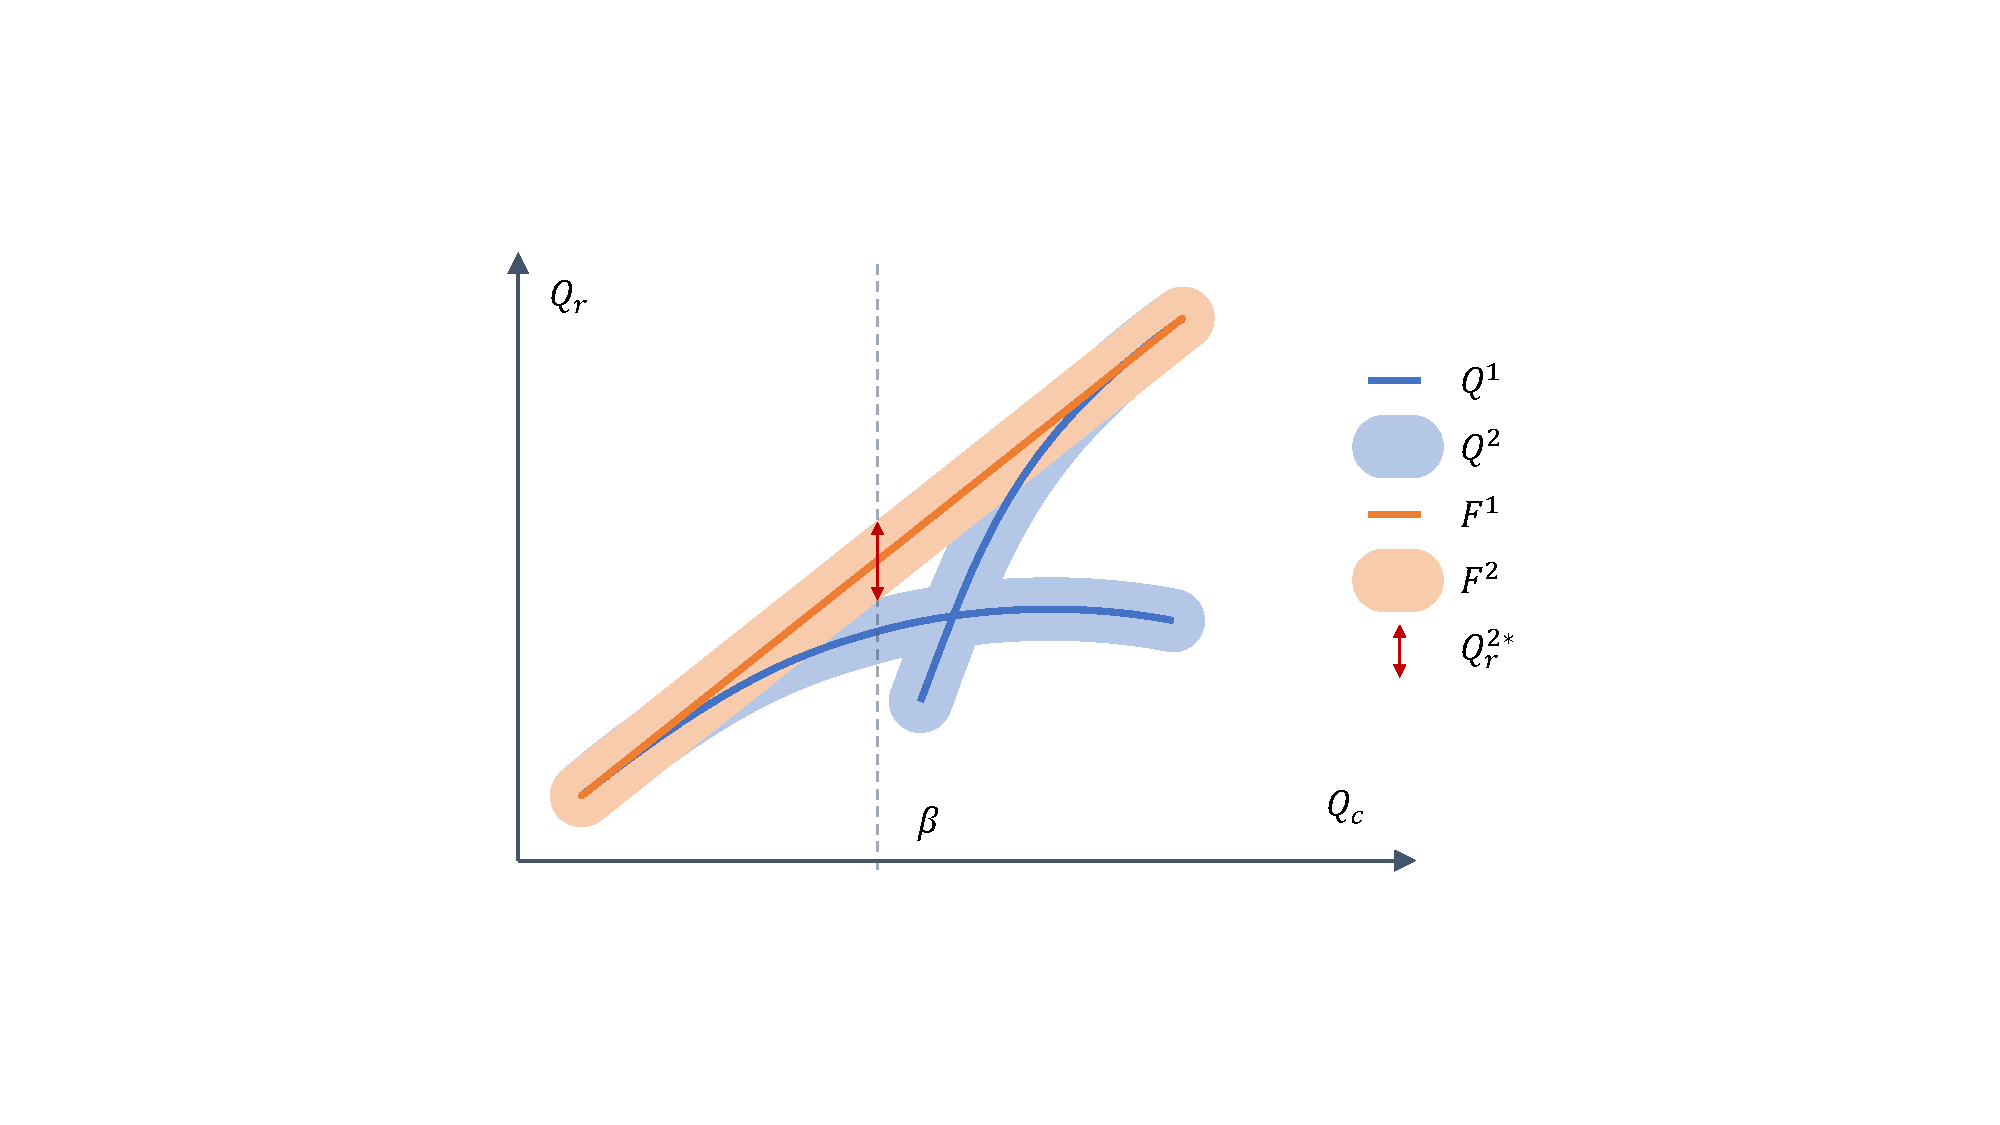
\includegraphics[trim=7cm 4cm 7cm 4cm, clip, width=0.7\textwidth]{img/contraction_lipschitz.pdf}
        \caption{We represent the range of possible solutions $\Qr[^{2\star}]$ for any $\oQ^2\in\text{Ball}(\oQ^1)$, given $\oQ_1\in\cL_\lambda$}
        \label{fig:contraction_lips_hull}
    \end{figure}

    \paragraph{Step 2}

    We want to show that if $\oQ\in\cL_{\discountfactor}$, $\cF$ is the graph of an $L$-Lipschitz function:
    \begin{equation}
        \label{eq:L-lip-set}
        \forall q^1,q^2\in\cF, |q_r^2-q_r^1| \leq |q_c^2-q_c^1|.
    \end{equation}

    Let $\oQ\in\cL_{\discountfactor}$ and $\os\in\ocS$, $\cF$ the corresponding top frontier of convex hull.
    For all $q^1,q^2\in\cF, \exists \lambda,\mu\in[0,1], q^{11},q^{12},q^{21},q^{22}\in \oQ(\os,\ocA)$ such that $q^1 = (1-\lambda)q^{11} + \lambda q^{12}$ and $q^2 = (1-\mu)q^{21} + \mu q^{22}$.
    Without loss of generality, we can assume $q_c^{11}\leq q_c^{12}$ and $q_c^{21}\leq q_c^{22}$. We also consider the worst case in terms of maximum $q_r$ deviation: $q_c^{12} \leq q_c^{21}$.
    Then the maximum increment $q_r^2-q_r^{1}$ is:
    \begin{align*}
        \|q^2_r-q^{1}_r\| &\leq \|q^{12}_r-q^{1}_r\| + \|q^{21}_r-q^{12}_r\| + \|q^{2}_r-q^{21}_r\| \\
        &= (1-\lambda)\|q^{12}_r-q^{11}_r\| + \|q^{21}_r-q^{12}_r\| + \mu\|q^{22}_r-q^{21}_r\| \\
        &\leq (1-\lambda)L\|q^{12}_c-q^{11}_c\| + L\|q^{21}_c-q^{12}_c\| + \mu L\|q^{22}_c-q^{21}_c\| \\
        &= L\|q^{12}_c-q^{1}_c\| + L\|q^{21}_c-q^{12}_c\| + L\|q^{2}_c-q^{21}_c\|\\
        &= L\|q^{2}_c-q^{1}_c\|.
    \end{align*}

    This can also be seen in \Cref{fig:contraction_lips_hull}: the maximum slope of the $\cF^1$ is lower than the maximum slope between two points of $\oQ^1$.

    \paragraph{Step 3}

    Let $\cF_1$ be a L-Lipschitz set as defined in \eqref{eq:L-lip-set}, and consider a ball $\text{Ball}(\cF_1,R)$ around it as defined in \eqref{eq:ball-set}.

    We want to bound the optimal reward value $\Qr[^{2\star}]$ under constraint $\Qc[^{2\star}] = \budget$ (regular case in \Cref{sec:proof_pi_hull} where the constraint is saturated), for any $\cF^2\in\text{Ball}(\cF_1,R)$. This quantity is represented as a red double-ended arrow in \Cref{fig:contraction_lips_hull}.

    Because we are only interested in what happens locally at $\Qc=\budget$, we can zoom in on \Cref{fig:contraction_lips_hull} and only consider a thin $\epsilon$-section around $\budget$. In the limit $\epsilon\rightarrow 0$, this section becomes the tangent to $\cF^1$ at $\Qc[^1]=\budget$. It is represented in \Cref{fig:contraction_lips_hull_slope}, from which we derive a geometrical proof:
    \begin{figure}[ht]
        \centering
        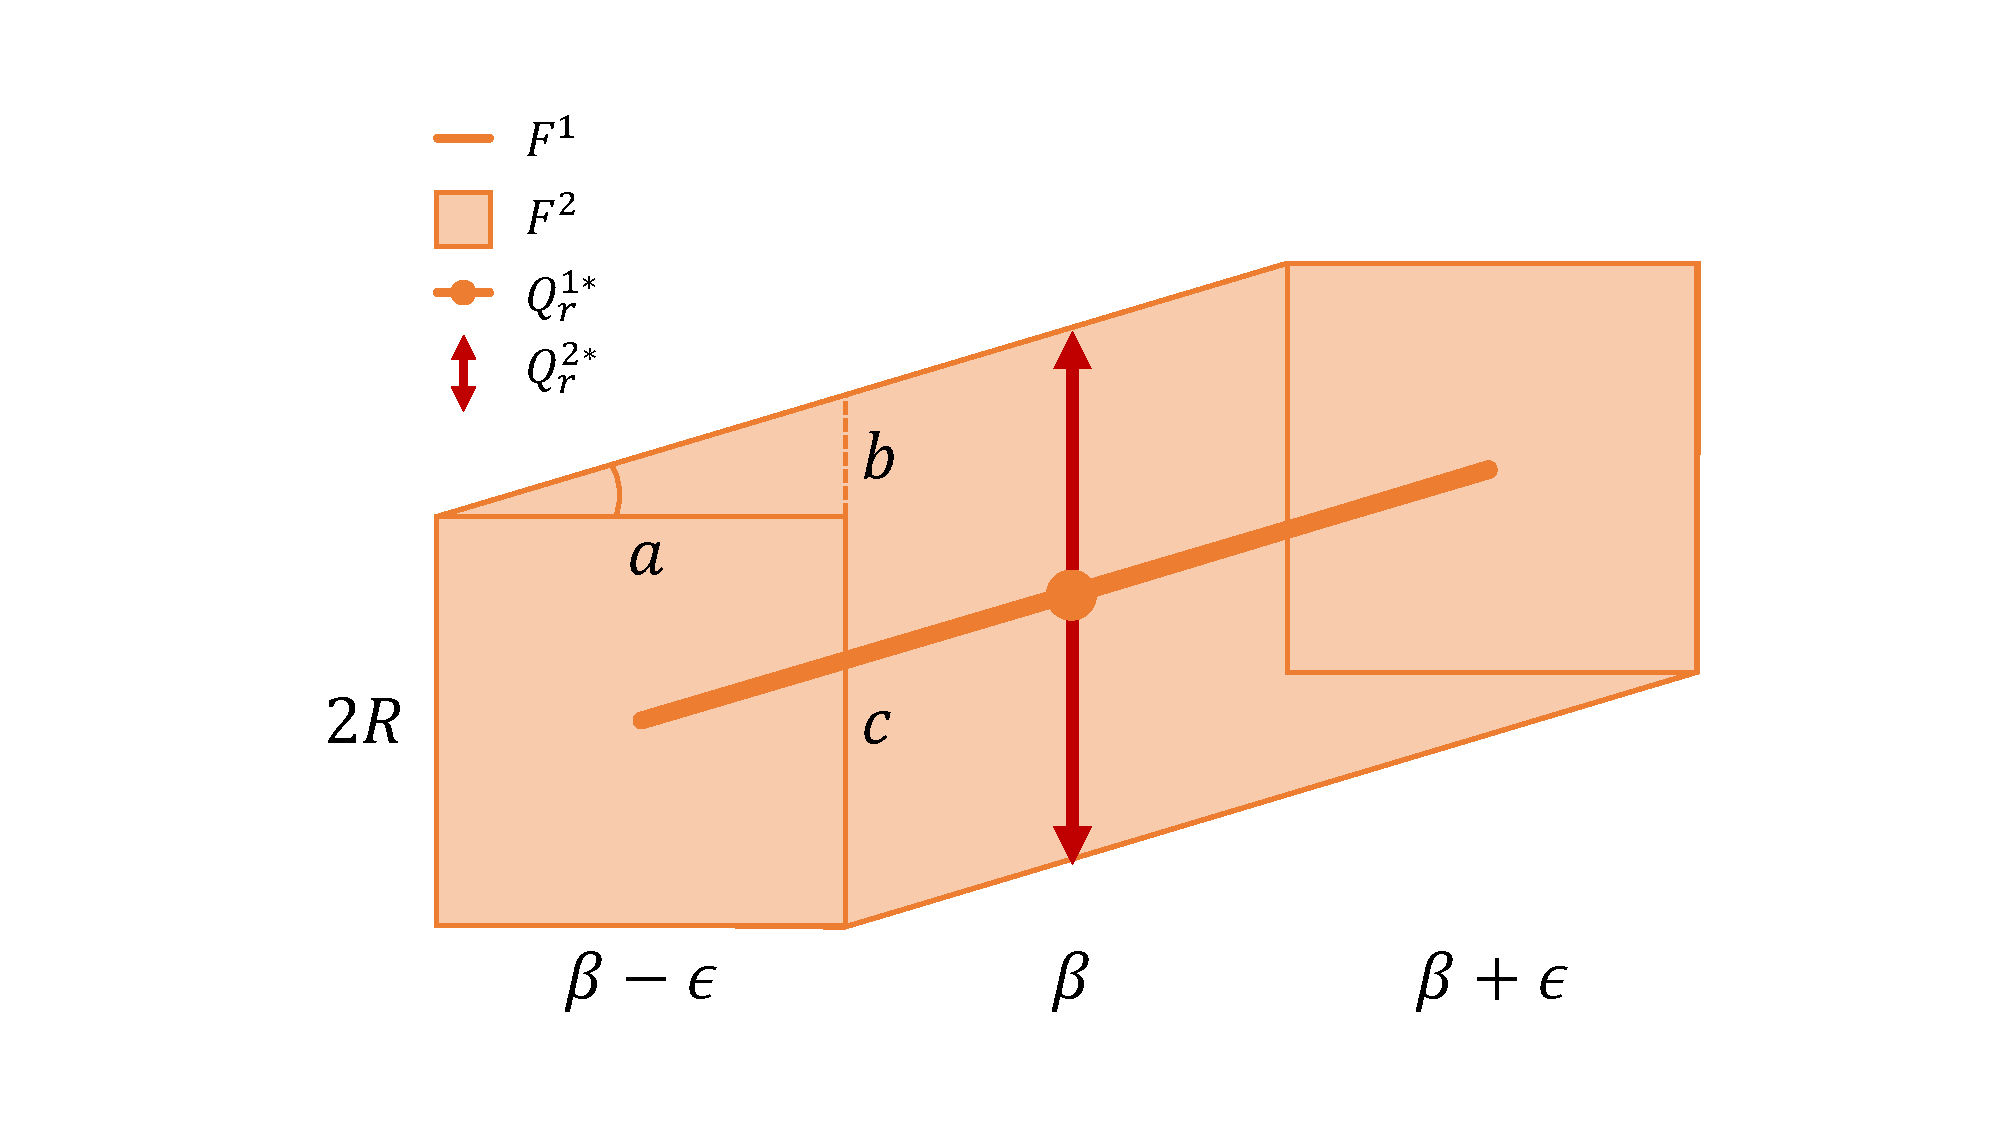
\includegraphics[trim=2cm 1cm 2cm 1cm, clip, width=0.7\textwidth]{img/contraction_lipschitz_slope.pdf}
        \caption{We represent a section $[\budget-\epsilon, \budget+\epsilon]$ of $\cF^1$ and $\text{Ball}(\cF^1, R)$. We want to bound the range of $\Qr[^{2\star}].$}
        \label{fig:contraction_lips_hull_slope}
    \end{figure}
    \begin{align*}
        \Delta \Qr[^{2\star}] &= b + c &\\
        & \leq La + c & \text{($\cF^1$ $L$-Lipschitz)}\\
        &= 2LR+2R = 2R(L+1).
    \end{align*}
    Hence,
    \begin{equation*}
        | \Qr[^{2\star}] - \Qr[^{1\star}]| \leq \frac{\Delta \Qr[^{2\star}]}{2} = R(L+1)
    \end{equation*}
    and $\Qc[^{1\star}] = \Qc[^{2\star}] = \budget$.
    Consequently, $ \|\oQ[^{2\star}] - \oQ[^{1\star}]\|_\infty \leq (L+1)R$.

    Finally, consider the edge case in \Cref{sec:proof_pi_hull}: the constraint is not active, and the optimal value is simply $\argmax_{q\in\cF} q^r$. In particular, since we showed that $\cF^2\in \text{Ball}(\cF^1, R)$, and since $\oQ[^{2\star}]\in \cF^2$, there exist $q^1\in \cF^1: \|\oQ[^{2\star}]-q^1\|_\infty\leq R$ and in particular $\oQ[^{1\star}]_r \geq q^1_r \geq \oQ[^{2\star}]_r - R$. Reciprocally, by the same reasoning, $\Qr[^{2\star}] \geq \Qr[^{1\star}] - R$. Hence, we have that $| \Qr[^{2\star}] - \Qr[^{1\star}]| \leq R \leq R(L+1).$

    \paragraph{Wrapping it up}

    We have shown that for any $\oQ^1,\oQ^2\in\cL_{\discountfactor}$,
    and all $\os\in\ocS$, $\cF^2\in\text{Ball}(\cF^1,\|\oQ^2-\oQ^1\|_\infty)$ and $\cF^1$ is
    the graph of a $L$-Lipschitz function with $L<1/\discountfactor - 1$.
    Moreover, the solutions of $\budgetedpolicy_\text{greedy}(\oQ^1)$ and $\budgetedpolicy_\text{greedy}(\oQ^2)$ at
    $\os$ are such that $ \|\oQ[^{2\star}] - \oQ[^{1\star}]\|_\infty \leq (L+1)\|\oQ^2-\oQ^1\|_\infty$.

    Hence, for all $\oa$,
    \begin{align*}
        \|\abo^{\star}\oQ^1(\os, \oa) - &\abo^{\star}\oQ^2(\os, \oa)\|_\infty \\
        &= \discountfactor\left\|\expectedvalueover{\os'\sim\augmentedtransition(\os'|\os,\oa)}
        \expectedvalueover{\oa'\sim\budgetedpolicy_\text{greedy}(\oQ^1)}\oQ^1(\os',\oa') -
        \expectedvalueover{\oa'\sim\budgetedpolicy_\text{greedy}(\oQ^2)}\oQ^2(\os',\oa')\right\|_\infty \\
        &= \discountfactor\left\|\oQ[^{2\star}] - \oQ[^{1\star}]\right\|_\infty \\
        &\leq \discountfactor(L+1)\|\oQ^2-\oQ^1\|_\infty.
    \end{align*}
    Taking the sup on $\ocS\ocA$,
    \begin{equation*}
        \|\abo^{\star}\oQ^1 - \abo^{\star}\oQ^2\|_\infty \leq \discountfactor(L+1)\|\oQ^1-\oQ^2\|_\infty
    \end{equation*}
    with $\discountfactor(L+1) < 1$.
    As a conclusion, $\abo^{\star}$ is a $\discountfactor(L+1)$-contraction on $\cL_{\discountfactor}$.
\end{proof}

%\subsection{\Cref{lemma:concavity}}

%\begin{proof}. Let $s,s'\in\cS, a\in\cA$.
%We first prove those results for $V_r^{\star}(s', \cdot)$

%\textbf{Non-decreasing}

%Consider $\beta_a^1 \leq \beta_a^2 \in \cB$.
%Any policy that satisfies the budget $\beta_a^1$ in $s'$ also satisfies $\beta_a^2$, so $\Pi_c(s', \beta_a^1) \subset \Pi_c(s', \beta_a^2)$. Hence, by taking the max over policies, $V_r^{\star}(s', \beta_a^1) \leq V_r^{\star}(s', \beta_a^2)$.
%Hence, $V_r^{\star}(s', \cdot)$ is non-decreasing.

%\textbf{Concave}

%By contradiction: assume that $V_r^{\star}(s', \cdot)$ is not concave, \ie there exist $\beta^1 < \beta^2\in \cB$ and $p\in(0, 1)$ such that $\beta^3 = (1-p)\beta^1 + p\beta^2$ verifies: $V_r^{\star}(s', \beta^3) < (1-p)V_r^{\star}(s', \beta^1) + pV_r^{\star}(s',\beta^2)$. By definition of $V^{\star}$, there must be $\pi_1,\pi_2\in\Pi^{\star}$ such that $V^{\star}(s', \beta^1) = V^{\pi_1}(s', \beta^1)$ and $V^{\star}(s', \beta^2) = V^{\pi_2}(s', \beta^2)$. 

%Define $\pi = (1-p)(\pi_1(\cdot, \beta^1), \pi_1) + p(\pi_2(\cdot, \beta^2), \pi_2)$. By linearity of $V^\pi$ with respect to $\pi$, we have that $V_c^\pi(s', \beta^3) = (1-p)V_c^{\pi_1}(s', \beta^1) + pV_c^{\pi_2}(s', \beta^2) \leq (1-p)\beta^1 + p\beta^2 = \beta^3$ since $\pi_1, \pi_2\in\Pi^{\star}(s')\subset\Pi_a(s')$, so $\pi$ respects the budget $\beta^3$. Moreover, we also have $V_r^\pi(s', \beta^3) = (1-p)V_r^{\pi_1}(s', \beta^1) + pV_r^{\pi_2}(s', \beta^2) > V_r^{\star}(s', \beta^3)$, which contradicts the definition of $V_r^{\star}$.

%Consequently, $V_r^{\star}(s', \cdot)$ is non-decreasing and concave. By \eqref{eq:bellman_expectation_Q} we see that $Q_r^{\star}(s,a,\cdot) = R_r(s,a) + \discount\expectedvalueover{s'}V_r^{\star}(s', \cdot)$  is too.


%\end{proof}

%\subsection{\Cref{lemma:tau_concavity}}


%\subsection{\Cref{lemma:pi_hull}}

%\td

%\begin{proof}
%If the estimates $q^c_0, q^c_1$ are accurate, then by construction and linearity of the expectation, the returned mixture policy has an expected total cost of $\expectedvalueover{a, \beta_a \sim\pi_\text{greedy}}Q_c(s, a, \beta_a) = \beta$ as desired in \eqref{eq:pi_greedy_constraint}. Because the $Q_r(s,a,\cdot)$ is concave and under its tangents, this mixture must have the largest $Q_r$ possible as required in \eqref{eq:pi_greedy_reward}. The special case of a tie $q_r^0 = q_r^1$ is considered, where we do minimise $Q_c$ as required in \eqref{eq:pi_greedy_cost}.
%\end{proof}


\subsection{Proof of \Cref{prop:bftq_pi_hull}}
\label{sec:proof_pi_hull}
\begin{definition}
	\begin{leftbar}[defnbar]
	Let $A$ be a set, and $f$ a function defined on $A$. We define
	
	\begin{itemize}
		\item the convex hull of $A$: $\cC(A) = \{\sum_{i=1}^p \lambda_i a_i: a_i\in A, \lambda_i\in\Real^+, \sum_{i=1}^p \lambda_i = 1, p\in\Natural\}$;
		\item the convex edges of $A$: $\cC^2(A) = \{\lambda a_1 + (1-\lambda)a_2: a_1, a_2\in A, \lambda\in[0, 1]\}$;
		\item Dirac distributions of $A$: $\dirac(A) = \{\dirac(a-a_0): a_0\in A\}$;
		\item the image of $A$ by $f$: $f(A) = \{f(a): a\in A\}$.
	\end{itemize}
\end{leftbar}
\end{definition}

\begin{proof}
Let $\os=(s,\budget)\in\ocS$ and $\oQ\in(\Real^2)^{\ocS\ocA}$. We recall the definition of $\budgetedpolicy_\text{greedy}$:
    \begin{subequations}
        \begin{align}
            \budgetedpolicy_\text{greedy}(\oa|\os; \oQ) &\in \argmin_{\rho\in\policies_r^{\oQ}} \expectedvalueover{\oa\sim\rho}\Qc(\os, \oa) \tag{\ref{eq:pi_greedy_cost}}\\
            \text{where }\quad\policies_r^{\oQ} = &\argmax_{\rho\in\cM(\ocA)} \expectedvalueover{\oa\sim\rho} \Qr(\os, \oa) \tag{\ref{eq:pi_greedy_reward}}\\
            & \text{ s.t. }  \expectedvalueover{\oa\sim\rho} \Qc(\os, \oa) \leq \budget \tag{\ref{eq:pi_greedy_constraint}}
        \end{align}
    \end{subequations}

    Note that any policy in the $\argmin$ in \eqref{eq:pi_greedy_cost} is suitable to compute $\abo^{\star}$.
    We first reduce the set of candidate optimal policies.
    Consider the problem described in \eqref{eq:pi_greedy_reward},\eqref{eq:pi_greedy_constraint}: it can be seen as a single-step \gls{CMDP} problem with reward $\reward=\Qr$ and cost $\constraint=\Qc$. By \citep[Theorem 4.4][]{Beutler1985}, we know that the solutions are mixtures of two deterministic policies. Hence, we can replace $\cM(\cA)$ by $\cC^2(\dirac(\ocA))$ in \eqref{eq:pi_greedy_reward}.

    Moreover, remark that:
    \begin{align*}
        \{\expectedvalueover{\oa\sim\rho} \oQ(\os,\oa):& \rho\in \cC^2(\dirac(\ocA))\} \\
        &= \{\expectedvalueover{\oa\sim\rho} \oQ(\os,\oa): \rho=(1-\lambda)\dirac(\oa-\oa_1)+\lambda\dirac(\oa-\oa_2), \oa_1,\oa_2\in\ocA, \lambda\in[0,1]\} \\
        &= \{(1-\lambda)\oQ(\os, \oa_1)+\lambda \oQ(\os, \oa_2), \oa_1,\oa_2\in\ocA, \lambda\in[0,1]\} \\
        &= \cC^2(\oQ(\os,\ocA))\}.
    \end{align*}

    Hence, the problem \eqref{eq:pi_greedy_reward}, \eqref{eq:pi_greedy_constraint} has become:
    \begin{equation*}
        \tilde{\policies}^{\Qr} = \argmax_{(q_r, q_c)\in\cC^2(\oQ(\os, \ocA))} q_r \quad\text{ s.t. }\quad q_c \leq \budget
    \end{equation*}
    and the solution of $\budgetedpolicy_\text{greedy}$ is $q^{\star}=\argmin_{q\in\tilde{\policies}^{\Qr}} q_c$.

    The original problem in the space of actions $\ocA$ is now expressed in the space of values $\oQ(\os, \ocA)$ (which is why we use $=$ instead of $\in$ before $\argmin$ here).

    We further restrict the search space of $q^{\star}$ following two observations:
    \begin{enumerate}
        \item $q^{\star}$ belongs to the \emph{undominated} points $\cC^2(\oQ^-)$:
        \begin{align}
            \label{eq:q_minus_undominated}
            \oQ^+ &= \{(q_c, q_r): q_c > q_c^{\pm} = \min_{q^+} q_c^+\text{ s.t. }q^+\in\argmax_{q\in \oQ(\os,\ocA)} q_r\}\\
            \oQ^- &= \oQ(\os,\ocA) \setminus \oQ^+.
        \end{align}
        Denote $q^{\star}$ = $(1-\lambda) q^1 + \lambda q^2$, with $q^1, q^2\in \oQ(\os,\ocA)$. There are three possible cases:
        \begin{enumerate}
            \item $q^1, q^2 \not\in \oQ^-$. Then $q_c^{\star} = (1-\lambda) q^1_c + \lambda q^2_c > q_c^{\pm}$. But then $q_c^{\pm} < q_c^{\star} \leq \budget$ so $q^{\pm}\in\tilde{\policies}^{\Qr}$ with a strictly lower $q_c$ than $q^{\star}$, which contradicts the $\argmin$.
            \item $q^1\in \oQ^-, q^2 \not\in \oQ^-$. But then consider the mixture $q^\top = (1-\lambda) q^1 + \lambda q^\pm$. Since $q_r^{\pm} \geq q_r^{2}$ and $q_r^{\pm} < q_r^{2}$, we also have $q^\top_r \geq q_r^{\star}$ and $q^\top_c < q_c^{\star}$, which also contradicts the $\argmin$.
            \item $q^1,q^2\in \oQ^-$ is the only remaining possibility.
        \end{enumerate}
        \item $q^{\star}$ belongs to the \emph{top frontier} $\cF$:
        \begin{equation}
            \label{eq:top-frontier}
            \cF_{\oQ} = \{q\in \cC^2(\oQ^-): \not\exists q'\in \cC^2(\oQ^-): q_c=q_c'\text{ and }q_r<q_r'\}.
        \end{equation}
        Trivially, otherwise q' would be a better candidate than $q^{\star}$.
    \end{enumerate}


    Let us characterise this frontier $\cF$. It is both:
    \begin{enumerate}
        \item the \emph{graph of a non-decreasing function}: $\forall q^1, q^2\in\cF$ such that $q_c^1\leq q_c^2$ then $q_r^1\leq q_r^2$.\\
        By contradiction, if we had $q_r^1 > q_r^2$, we could define $q^\top = (1-\lambda)q^1 + \lambda q^\pm$ where $q^\pm$ is the dominant point as defined in \eqref{eq:q_minus_undominated}. By choosing $\lambda=(q^2_c-q^1_c)/(q^\pm_c-q^1_c)$ such that $q^\top_c = q_c^2$, then since $q_r^\pm \geq q_r^1 > q_r 2$ we also have $q^\top_r > q_r^2$ which contradicts $q^2\in\cF$.
        \item the \emph{graph of a concave function}: $\forall q^1, q^2, q^3\in\cF$ such that $q_c^1\leq q_c^2 \leq q_c^3$ with $\lambda$ such that $q^2_c = (1-\lambda)q^1_c + \lambda q^3_c$, then $q_r^2 \geq (1-\lambda)q_r^1 + \lambda q_r^3$.\\
        Trivially, otherwise the point $q^\top = (1-\lambda)q^1 + \lambda q^3$ would verify $q^\top_c=q^2_c$ and $q^\top_r > q^2_r$, which would contradict $q^2 \in\cF$.
    \end{enumerate}

    We denote $\cF_{\oQ} = \cF \cap \oQ$. Clearly, $q^{\star}\in\cC^2(\cF_{\oQ})$: let $q^1, q^2\in \oQ^-$ such that $q^{\star} = (1-\lambda)q^1 + \lambda q^2$. First, $q^1, q^2\in \oQ^-\subset\cC^2(\oQ^-)$. Then, by contradiction, if there existed $q^{1'}$ or $q^{2'}$ with equal $q_c$ and strictly higher $q_r$, again we could build an admissible mixture $q^{\top}=(1-\lambda)q^{1'}  + \lambda q^{2'}$ strictly better than $q^{\star}$.

    $q^{\star}$ can be written as $q^{\star} = (1-\lambda)q^1 + \lambda q^2$ with $q^1, q^2\in\cF_{\oQ}$ and, without loss of generality, $q^1_c \leq q^2_c$.

    \paragraph{Regular case}

    There exists $q^0\in\cF_{\oQ}$ such that $q^0_c \geq \budget$. Then $q^1$ and $q^2$ must flank the budget: $q_c^1 \leq \budget \leq q_c^2$. Indeed, by contradiction, if $q_c^2 \geq q_c^1 > \budget$ then $q_c^{\star} > \budget$ which contradicts $\policies_r^{\oQ}$. Conversely, if $q_c^1 \leq q_c^2 < \budget$ then $q^{\star} < \budget \leq q^0_c$, which would make $q^{\star}$ a worse candidate than $q^\top=(1-\lambda)q^{\star} + \lambda q^0$ when $\lambda$ is chosen such that $q_c^\top=\budget$, and contradict $\policies_r^{\oQ}$ again.

    Because $\cF$ is the graph of a non-decreasing function, $\lambda$ should be as high as possible, as long as the budget $q^{\star}\leq\budget$ is respected. We reach the highest $q_r^{\star}$ when $q^{\star}_c=\budget$, that is: $\lambda=(\budget-q_c^1)/(q_c^2-q_c^1)$.

    It remains to show that $q^1$ and $q^2$ are two successive points in $\cF_{\oQ}$: $\not\exists q\in\cF_{\oQ}\setminus\{q^1, q^2\}: q^1_c \leq q_c \leq q^2_c$. Otherwise, as $\cF$ is the graph of a concave function, we would have $q_r \geq (1-\mu)q_r^1 + \mu q_r^2$. $q_r$ cannot be strictly greater than $(1-\mu)q_r^1 + \mu q_r^2$ which would contradict $q^{\star}$, but it can still be equal, which means the tree points $q, q^1, q^2$ are aligned. In fact, every points aligned with $q^1$ and $q^2$ can also be used to construct mixtures resulting in $q^{\star}$, but among these solutions we can still choose $q^1$ and $q^2$ as the two points in $\cF_{\oQ}$ closest to $q^{\star}$.

    \paragraph{Edge case}

    $\forall q\in\cF_{\oQ}, q_c < \budget$. Then  $q^{\star} =  \argmax_{q\in\cF} q_r = q^\pm =  \argmax_{q\in \oQ^-} q_r$.
\end{proof}


%\begin{proof}
%First, a straightforward proof by induction shows that for all $k\in\Natural$, $Q_k$ computed at iteration $k$ of either \Cref{alg:bvi} or \Cref{alg:bftq} is concave non-decreasing with respect to $\beta_a$: the initialisation is trivial from $Q_0 = 0$, and the heredity stems from \Cref{lemma:tau_concavity}.
%\end{proof}


% \subsection{Decomposition Lemma}

% \begin{lemma}
%     For any sequence real valued functions $f_1,\ldots,f_n$ and any real number $c$, we have
%     \[
%         \begin{array}{lcl}
%             \underbrace{\max\limits_{\sum_i x_i \leq c}\sum_j f_j(x_j)}_{(a)} & \quad{}=\quad{} & \underbrace{\max\limits_{\sum_i c_i \leq c}\left(\sum_j\max\limits_{x\leq c_j} f_j(x)\right)}_{(b)}\\
%         \end{array}
%     \]
% \end{lemma}

% \begin{proof}
%     Let us first show that $(a)\leq(b)$.
%     By definition of the maximum on a set, for any $f_j$ and any $c_j$ we have
%     $\max\limits_{x\leq c_j} f_j(x) \geq f_j(c_j)$.
%     Hence, by replacing these terms in $(b)$ we get:
%       \[
%     \begin{array}{lcl}
%         \max\limits_{\sum_i c_i \leq c} \sum_j f_j(c_j) & \quad{}\leq\quad{} & \max\limits_{\sum_i c_i\leq c}\left(\sum_j \max\limits_{x_j\leq c_j} f_j(x_j)\right)\\
%     \end{array}
%     \]
%     The left hand side of this inequality is just a rewriting of $(a)$ with different dummy variables names.

%     Let us show now that $(a) \geq (b)$.
%     Let $\hat{x}_1,\ldots,\hat{x}_n, \hat{c}_1, \ldots \hat{c}_n$ be a realisation (argmax) of $(b)$.
%     By definition of $(b)$'s feasible set, we have $\sum_i\hat{c}_i \leq c$ and for any $i$: $\hat{x}_i\leq \hat{c}_i$.
%     Because $\sum_i\hat{x}_i\leq \sum_i\hat{c}_i \leq c$, the tuple $(\hat{x}_1, \ldots \hat{x}_n)$ is also a feasible value for $(a)$. And, by definition of the maximum on a set: $(a) = \max\limits_{\sum_i x_i \leq c} \sum_j f_j(x_j) \geq \sum_j f_j(\hat{x}_j) = (b)$.
% \end{proof}

%\section{Risk-Sensitive Exploration}
%\label{sec:risk-sensitive-supp}
%We recall the Risk-Sensitive Exploration in %\Cref{alg:risk-sensitive-exploration}:
%\begin{algorithm}[ht]
\DontPrintSemicolon
\KwData{An environment, a BFTQ solver, $W$ CPU workers}
\KwResult{A batch of transitions $\cD$}
$\cD\leftarrow\emptyset$\;
\For{each intermediate batch} {
split episodes between $W$ workers\;
\For(\tcp*[f]{run this loop on each worker in parallel}){each episode in batch}{
sample initial budget $\beta\sim\mathcal{U}(\mathcal{B})$.\;
\While{episode not done}{
update $\epsilon$ from schedule.\;
sample $z\sim\mathcal{U}([0, 1])$.\;
\lIf{$z < \epsilon$}{sample $(a, \beta_a)\sim\mathcal{U}(\Delta_{\cA\cB})$.\tcp*[f]{Explore}}
\lElse{sample $(a, \beta_a)\sim\pi_\text{greedy}(a, \beta_a|s, \beta; Q^{\star})$.\tcp*[f]{Exploit}}
append transition $(s, \beta, a, \beta_a, R, C, s')$ to batch $\mathcal{D}$.\;
step episode budget $\beta \leftarrow \beta_a$
}
}
$\pi_\text{greedy}(\cdot\sim; ~Q^{\star}) \leftarrow\texttt{BFTQ}(\cD)$.
}
\Return{the batch of transitions $\cD$}
\caption{Risk-sensitive exploration}
\label{algo:risk-sensitive-exploration}
\end{algorithm}
